%
% $XORP: xorp/docs/windows_port/windows_port.tex,v 1.7 2009/01/09 19:21:02 jtc Exp $
%

\documentclass[11pt]{article}

%\usepackage[dvips]{changebar}

\usepackage{subfigure}
\usepackage{fullpage}
\usepackage{setspace}
\usepackage{times}
\usepackage{latexsym}
\usepackage{epsfig}
\usepackage{ifpdf}
%\usepackage{graphicx}
\usepackage{xspace}
\usepackage{color}
\usepackage{amsmath}
\usepackage{rotating}
\usepackage{moreverb}
\usepackage{listings}
\usepackage{alltt}
\usepackage{stmaryrd}
\usepackage{url}
%\usepackage{hyperref}
%\usepackage{tabularx}
%\usepackage[dvipdf]{graphics}
%\usepackage[dvips]{graphicx}
%\usepackage{xorp}

% The following is needed in order to make the code compatible
% with both latex/dvips and pdflatex.
%\ifx\pdftexversion\undefined
%\usepackage[dvipdf]{graphicx}
%\else
\usepackage{graphicx}
%\DeclareGraphicsRule{*}{mps}{*}{}
%\fi

\definecolor{gray}{rgb}{0.5,0.5,0.5}
\newcommand{\etc}{\emph{etc.}\xspace}
\newcommand{\ie}{\emph{i.e.,}\xspace}
\newcommand{\eg}{\emph{e.g.,}\xspace}
%\newcommand{\comment}[1]{{\color{gray}[\textsf{#1}]}}
%\newcommand{\comment}[1]{}

% Changebar stuff
% \newenvironment{colorcode}{\color{blue}}{}
% \renewcommand{\cbstart}{\begin{colorcode}}
% \renewcommand{\cbend}{\end{colorcode}}

% \pagestyle{empty}

\begin{document}

\title{XORP Windows Support Overview \\
\vspace{1ex}
Version 1.7}
\author{ XORP, Inc. and individual contributors		\\
         {\it http://www.xorp.org/}			\\
	 {\it xorp-users@xorp.org}
}
\date{April 29, 2010}

\maketitle


%%%%%%%%%%%%%%%%%%%%%%%%%%%%%%%%%%%%%%%%%%%%%%%%%%%%%%%%%%%%%%%%%%%%%%%
\section{Introduction}

As of XORP 1.7, Microsoft Windows is no longer supported.  This
document is kept for posterity's sake.

This document provides an overview of XORP's support for Microsoft Windows.
Much of XORP's internal library implementation is specifically targeted
at UNIX-like operating environments. Here, we summarize the steps involved
in the initial port, as well as describing how the Windows support code
functions in detail. It is aimed at developers coming from a Windows
development background.
To summarize current Windows support at the time of writing:
\begin{itemize}
 \item IPv4 unicast routing is fully supported.
 \item IPv6 control plane traffic appears to work under Windows
``Longhorn'' Server, however, access to the IPv6 forwarding plane
is not supported.
 \item The multicast forwarding plane is not supported. The architecture
for this in Windows differs significantly from other operating systems.
\end{itemize}

XORP is composed of around 360,000
\footnote{Measured using C and C++ Code Counter: \url{http://cccc.sourceforge.net/}}
actual lines of code at the time of writing.
Prior to the port, the code was only portable amongst
a small subset of UNIX-like operating systems. As such, the effort
considerably improved the portability of the XORP code base as a whole.

The Windows port presented the XORP team at ICSI with a significant technical
challenge which was met successfully.
A XORP router  was
demonstrated in July 2005, at Microsoft Research in Redmond.
It was hosted on commodity PC hardware, running Windows Server 2003,
and successfully handled a full eBGP feed of around 120,000 IPv4 route prefixes.

%%%%%%%%%%%%%%%%%%%%%%%%%%%%%%%%%%%%%%%%%%%
\subsection{The initial port}

Work on the initial port of XORP to Microsoft Windows began
in February 2005. An iterative, bottom-up approach was used, where a build attempt
was made in several stages with different tool chains at each stage. As the
port progressed, the error feedback from the previous stage was used to rewrite
areas of the code base which did not compile or which were significantly
incompatible with Windows systems programming idioms.

%%%%%%%%%%%%%%%%%%%%%%%%%%%%%%%%%%%%%%%%%%%
\subsection{Constraints}

XORP is subject to certain portability constraints. At the moment,
whenever a new platform is targeted, the following constraints apply at a minimum:
\begin{itemize}
 \item The ability to run the GNU {\tt configure} script.
       This requires a POSIX compliant shell.
 \item The ability to read and manipulate the target's IPv4 forwarding plane.
 \item The compiler must support variadic macros, either in a manner which is
C99 compatible, or with GNU extensions.
 \item Changes to support the new platform should be minimally intrusive.
\end{itemize}


%%%%%%%%%%%%%%%%%%%%%%%%%%%%%%%%%%%%%%%%%%%
\subsection{64-bit forward compatibility}

Whilst every effort has been made to use APIs which are forward compatible
with operation under Win64, it has not been possible to test XORP's
native operation on 64-bit Windows systems due to the lack of a MinGW
toolchain for these systems. The Win32 binaries have however been
compiled and run on 64-bit systems on a purely experimental basis.

%%%%%%%%%%%%%%%%%%%%%%%%%%%%%%%%%%%%%%%%%%%%%%%%%%%%%%%%%%%%%%%%%%%%%%%
\section{Port stages}

This section describes each evolutionary stage of the Windows port,
in terms of the tool chain used.

%%%%%%%%%%%%%%%%%%%%%%%%%%%%%%%%%%%%%%%%%%%
\subsection{Cygwin}

In the beginning,
Cygwin
\footnote{\url{http://www.cygwin.com/}},
a UNIX-like environment for Windows,
was used as the first stage:
\begin{itemize}
  \item It provides an emulated, Windows-hosted GNU {\tt gcc} and {\tt g++} tool chain.
  \item It provides a POSIX-like emulation environment.
  \item It is {\em not} a Windows subsystem
        \footnote{\url{http://technet.microsoft.com/en-us/library/cc767884.aspx}}
  \item The binaries it produces require the use of the {\tt CYGWIN.DLL} runtime DLL,
        which provides the POSIX-like emulation.
  \item A POSIX-compliant shell is available, capable of running GNU {\tt configure} scripts.
\end{itemize}

The objective at this point was simply to get as much of the XORP code base
to compile as possible, in a self-hosting manner, on Windows.
Cygwin's runtime libraries are mostly compatible with POSIX and C99 standards,
making this an easier task than it would otherwise be.

However, due to the lack of access to native Windows APIs, including {\tt CreateProcess()},
the XORP Router Manager and CLI could not be ported at this stage.
Furthermore, the IPv4 forwarding table was not accessible from the FEA.
Only IPv4 networking facilities are supported by Cygwin, using a
limited subset of the Berkeley Socket APIs. There is no access to the
forwarding plane.

The use of {\tt CYGWIN.DLL} was not compatible with XORP's license at the
time of the port. The DLL itself is licensed under the GNU General Public License version 2,
{\em not} the ``Library'' version of this license. A general release of this
development code would have tainted all XORP binaries with the GPLv2 license.

Porting to Cygwin, however, allowed several more general problems in the code
base to be found and resolved, in preparation for the next stage.

%%%%%%%%%%%%%%%%%%%%%%%%%%%%%%%%%%%%%%%%%%%
\subsection{MinGW}

The next stage in the evolution of the port was to adopt the use
of Minimalist GNU for Windows (MinGW)
\footnote{\url{http://www.mingw.org/}},
a freely available port of
the GNU {\tt gcc} tool chain capable of producing native Win32 binaries:
\begin{itemize}
 \item It provides a native, Windows-hosted GNU {\tt gcc} and {\tt g++} tool chain.
 \item It does {\em not} provide a POSIX emulation environment.
 \item It ships its own version of the Microsoft Windows SDK
       headers and libraries, {\tt w32api}, which is compatible with {\tt gcc}.
 \item The binaries it produces use the Windows system native runtime, {\tt MSVCRT.DLL}
       \footnote{This is the C runtime library used by Windows system components;
                 it is not part of Microsoft Visual C++.}.
 \item It is {\em not} a Windows subsystem. However, the binaries it produces
        are clients of the Win32 subsystem.
\end{itemize}

Porting XORP to MinGW provided the project with the necessary means to use
native Windows system APIs.
Minimalist access to the IPv4 forwarding plane was now possible through the
IP Helper API, {\tt IPHLPAPI.DLL}.

Redistribution of binaries produced with MinGW is compatible with the Microsoft
End-User License Agreement. There are no additional requirements for the binaries
which are shipped, as the runtime DLL used is part of Windows itself, thus
resolving the incompatibility which existed between Cygwin and the
XORP license at that time.


%%%%%%%%%%%%%%%%%%%%%%%
\subsubsection{Windows SDK header support}

A caveat of using MinGW is that it does not benefit from Microsoft's
ongoing support, as regards SDK headers and libraries; it is purely dependent
upon user contributions. Microsoft's SDKs are targeted at Microsoft-compatible
compilers, as such they use compiler pragmas which are not compatible with
the GNU {\tt gcc} or {\tt g++} compilers. MinGW therefore ships its own SDK-like package
known as {\tt w32api}.

%%%%%%%%%%%%%%%%%%%%%%%
\subsubsection{GNU {\tt configure} capability}

Whilst the use of MinGW satisfied the requirement that a {\tt gcc}-compatible compiler be used,
it did not satisfy the requirement to be able to run GNU {\tt configure}.

However, there is a UNIX-like environment built on MinGW, called
MSYS\footnote{\url{http://www.mingw.org/wiki/msys}}, which
contains a POSIX-compliant shell capable of running GNU {\tt configure}. By installing
an additional package, {\tt msysDTK}, it is possible to run versions of the GNU
{\tt automake}, {\tt autoconf} and {\tt libtool} tools which are specifically customized for
the MinGW and MSYS environments.

The MSYS tools use a library of their own which is derived from Cygwin, however,
this is completely separate from Cygwin itself, and is not used by MinGW compiled processes,
which are fully fledged Win32 subsystem processes.

%%%%%%%%%%%%%%%%%%%%%%%
\subsubsection{C99 and POSIX compatibility}

It was therefore possible, by using the combination of MinGW and MSYS, to begin
porting XORP to a native Windows runtime environment. This approach,
however, has problems of its own.

Unlike Cygwin, MinGW has no POSIX emulation capability. There is a very thin veneer
of C99 and POSIX glue, in the form of various library functions.
The Windows system runtime, {\tt MSVCRT.DLL} supplies emulations of certain POSIX
or C runtime functions, and macros, as a convenience. Unfortunately, not all of these
behave identically to their counterparts in the UNIX environments.

One example which stands out is Microsoft's implementation of
the {\tt snprintf()} C string formatting function. The XRL layer has a strong, indirect
dependency on this function, and it behaves quite differently in terms of
its return value. A work around for this can be seen in {\tt libxorp/c\_format.cc}.

The {\tt -DNO\_OLDNAMES} preprocessor definition can be used to omit some of these definitions
from the MinGW SDK headers. XORP's use of names affected by this definition applies
mostly to file and directory access.

%%%%%%%%%%%%%%%%%%%%%%%
\subsubsection{MinGW port evolution}

The evolution of the MinGW based port has therefore followed three stages:
\begin{itemize}
 \item MinGW without {\tt -DNO\_OLDNAMES}.

The initial stage, used to wean XORP away from the dependencies on the Cygwin
environment to compile, and the most labor intensive stage of the porting process.

 \item MinGW with {\tt -DNO\_OLDNAMES}.

An intermediate stage, used to wean XORP code onto using the POSIX-like
file I/O routines shipped in {\tt MSVCRT.DLL}.

At this point in development, use of the {\tt XorpFd} class was tightened, in order to detect
programmer error which might result from confusing the use of the POSIX
file descriptor type {\tt int} with the Windows type {\tt HANDLE}.

 \item MinGW without {\tt -DNO\_OLDNAMES}.

The final stage of the port, used to simplify some of the header file glue
required by the Windows port, as the use of {\tt -DNO\_OLDNAMES} was found to clash
with some of the Multiple Provider Router (MPR) header files in the Windows SDK.
\end{itemize}

%%%%%%%%%%%%%%%%%%%%%%%%%%%%%%%%%%%%%%%%%%%%%%%%%%%%%%%%%%%%%%%%%%%%%%%
\section{Architectural Overview}

This section summarizes the main changes in the XORP architecture which
were made to accomodate Windows systems.
XORP was initially developed on the FreeBSD platform. This heritage
is reflected in the design and implementation of the {\tt EventLoop}
and {\tt SelectorList} classes in the main XORP class library,
{\tt libxorp}. FreeBSD has a history of following POSIX standards
fairly closely, therefore it has been a good choice for a reference
platform to date.

For a broader overview of the issues involved in capturing I/O
in object-oriented design patterns, please refer to \cite{schmidt:1999:AOA}.

\subsection{Portable I/O interfaces}

All I/O in XORP is event driven.
The {\tt AsyncFileReader}, {\tt AsyncFileWriter} and {\tt BufferedAsyncReader}
classes do not provide ``true'' asynchronous I/O
facilities; rather, they each capture an {\tt Adaptor}
design pattern, for building C++ event-driven I/O
facilities.

The {\tt EventLoop}
\footnote{Section 5, ``The main loop'', \cite{xorp:xorpdev_101}.}
class captures a {\tt Facade} pattern, for access to timer and
event-driven I/O facilities.
The interface is independent of the underlying operating system.
Each I/O class interacts with {\tt EventLoop} to register notifications
of pending I/O events.

\begin{figure}
 \centering
 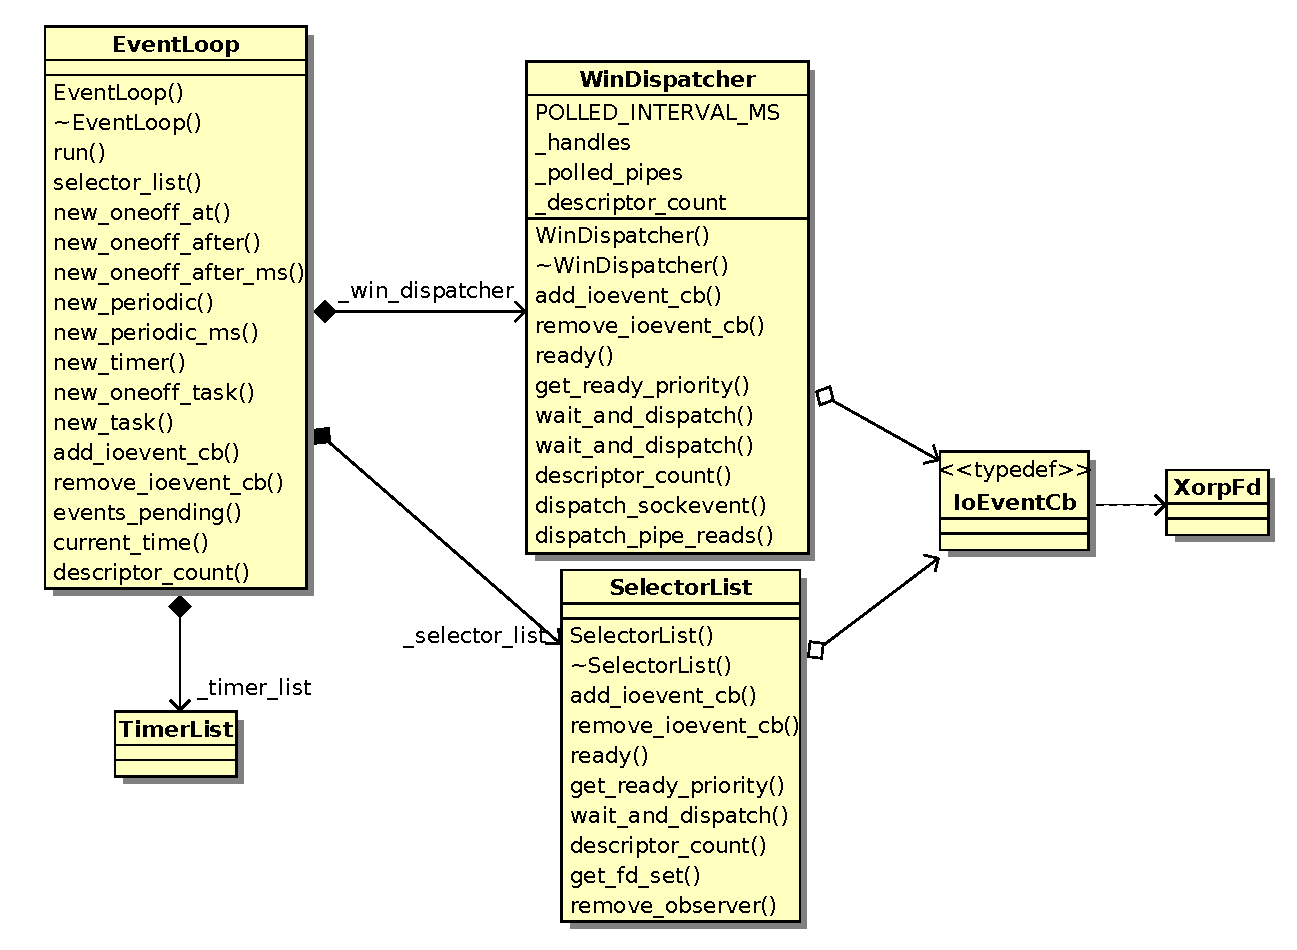
\includegraphics[scale=0.5,bb=0 0 622 456]{figs/windispatcher}
 % windispatcher.pdf: 622x456 pixel, 72dpi, 21.94x16.09 cm, bb=0 0 622 456
 \caption{UML class diagram of portable I/O facilities}
\end{figure}

Historically, XORP only supported UNIX-like systems. Therefore,
the design of the I/O facilities is layered on top of
POSIX non-blocking I/O, as they are natively supported by such systems.

An advantage of this approach is that I/O operations are inherently
self-serializing. The complexity of I/O multiplexing has been delegated
to the kernel, by relying on the atomicity of each POSIX system call.
Explicit locking is therefore not required in
XORP processes. Parallelism within UNIX-like kernels is a wholly
separate topic, and is outside the scope of this document.

\subsection{POSIX I/O implementation}

The {\tt EventLoop} contains an instance of {\tt SelectorList},
which encapsulates POSIX {\tt select()} based I/O multiplexing
in a C++ class.
The {\tt select()} system call
is used as it is portable between POSIX systems.
The POSIX I/O model in XORP makes the following assumptions:
\begin{itemize}
 \item Processes run in a single primary thread.
 \item The operating system supports POSIX ``non-blocking'' I/O operations.
 \item The operating system will serialize I/O on behalf of the process.
 \item Notifications of I/O events are {\em level-triggered} interrupts
       \footnote{This analogy is borrowed from digital logic design.}.
\end{itemize}

The implementation of {\tt SelectorList} can be considered to follow
the {\tt Reactor} object-oriented design pattern \cite{schmidt:reactor}.

\subsection{Windows I/O implementation}

The APIs available for I/O across the Windows system reflect the
Windows kernel's different design philosophy from that of UNIX.
Serialization is the responsibility of the user-space application,
as the kernel is intended to run with a high degree of parallelism.
As such, the Windows APIs for I/O are almost all implemented to block
the calling thread.
The Windows I/O model in XORP makes the following assumptions:
\begin{itemize}
 \item Win32 processes may contain multiple threads.
 \item Threads in the Win32 subsystem are implemented as
       a thin veneer on top of Windows kernel threads.
       These are treated as being cheap and easily available
       \footnote{This is reflected in the logo art for the Windows NT 4.0 release.}.
 \item The operating system {\em does not} support POSIX ``non-blocking'' I/O operations.
 \item The operating system {\em does not} serialize I/O on behalf of the process,
       unless alternative APIs are used.
 \item Notifications of I/O events are {\em edge-triggered} interrupts.
\end{itemize}

The implementation of {\tt WinDispatcher} can also be considered to capture
the {\tt Reactor} pattern.

Should threading support ever be required within the XORP programming model,
the design assumptions behind the EventLoop will need to be revisited.
The UNIX design philosophy persists to this day in XORP's reference
platforms.

The use of Windows asynchronous I/O primitives, \eg I/O completion ports
\footnote{\url{http://technet.microsoft.com/en-us/sysinternals/bb963891.aspx},}
has been considered for XORP, but was ruled out as it effectively meant
re-architecting the entire I/O model to support ``true'' asynchronous I/O.
An example of a design pattern which captures the requirements
of asynchronous I/O is the {\tt Proactor} pattern \cite{schmidt:coplien_pattern_1995}.

\subsection{I/O software interrupts}

The {\tt EventLoop} has responsibility for I/O event dispatch within XORP processes.
As a result of the difference in I/O strategies between UNIX-like kernels, and the
Windows kernel, the disposition of I/O events is correspondingly different.
Here, we compare {\tt WSAEnumNetworkEvents()} with
{\tt select()} in the context of socket I/O notifications:

\begin{center}
\begin{minipage}[0]{12cm}
\begin{tabular}{ | l | l | l | l | }
\hline

Multiplexing API & Read & Write & Exception \\ \hline\hline

{\tt select()} &
Level &
Level
\footnote{{\tt select()} indicates that a given file descriptor is writable
every time it is called.} &
Level \\

{\tt WSAEnumNetworkEvents()}
\footnote{The ``signalled'' condition is cleared if a Windows Event object is supplied as an argument.}
\footnote{One, and only one, indication will be returned that a previously posted write to a socket has completed,
or that a socket now has inbound readable data.}
&
Edge
&
Edge
&
Edge
\footnote{Error returns from previous Winsock I/O calls are in fact
dispatched inline with the event code corresponding to the
previously posted operation.} \\ \hline
\end{tabular} 
\end{minipage}
\end{center}

These multiplexing functions effectively poll for the
status of {\em software interrupts} on each file handle
provided as arguments.
As will be seen further on in the documentation for
{\tt WinDispatcher}
itself,
this table does not provide the full picture, as a number of other
work arounds are used there to account for the
differences in Windows I/O facilities.

The interrupts generated
by the POSIX {\tt select()} call are {\it level-triggered}; the change
in state persists in the time domain, \ie an event
condition on a POSIX file descriptor will persist between subsequent
calls to {\tt select()}, until the I/O is serviced.
With {\tt select()}, a read event persists until data is no longer
readable from the socket.

The interrupts generated by the Windows kernel API {\tt WaitForMultipleObjects()},
and the Winsock 2 API {\tt WSAEventSelect()}, are {\it edge-triggered}; the
change in state happens only once in the time domain and does not persist.
If an I/O event is not dispatched immediately upon return from the
multiplexing function in use, the event state will {\em not} be preserved
by the underlying operating system.

Workarounds for these key differences in behaviour are described
further on, in the documentation for the {\tt AsyncFileReader} and
{\tt AsyncFileWriter} classes.

%%%%%%%%%%%%%%%%%%%%%%%%%%%%%%%%%%%%%%%%%%%%%%%%%%%%%%%%%%%%%%%%%%%%%%%
\section{Global scope changes}

This section summarizes the changes to the XORP code base,
necessary for Windows support, which affected the global C and C++
identifier scope.

The bulk of the changes to support Microsoft Windows were checked into the
original XORP CVS repository on December 21, 2005.

To discover and explore
areas of the source tree which have been conditionalized for Windows support,
the reader may wish to use a source browsing application,
{\eg Red Hat Source Navigator}, and peform a search for references to
the preprocessor conditional
{\tt HOST\_OS\_WINDOWS}.

%%%%%%%%%%%%%%%%%%%%%
\subsection{GNU {\tt configure} changes}

XORP is normally built with a fairly rigorous set of compiler warning flags.
Unfortunately, these warnings are not compatible with the MinGW system headers,
or the {\tt w32api} headers.

In the Windows SDKs as normally shipped by Microsoft, this issue is addressed
by the use of several compiler pragmas specific to Microsoft Visual C++ and 
various compatible Windows-hosted compiler tool chains. In many cases,
compiler vendors, \eg Borland and Watcom, ship versions of the Microsoft SDKs
specifically tailored to the idiosyncracies of their own compilers.

These pragmas are not present in MinGW or the {\tt w32api}. Therefore, the GNU
{\tt configure} script for XORP specifically removes the following compiler
warning flags to enable the compiler to be built:
\begin{itemize}
 \item {\tt -Wmissing-declarations}
 \item {\tt -Wpointer-arith}
 \item {\tt -Wstrict-prototypes}
 \item {\tt -Wcast-align}
\end{itemize}

The {\tt configure} script is also responsible for detecting various properties
of the networking stack as seen by the build environment. Originally these
were part of {\tt configure.in} itself, however, as complexity grew, these tests
were parceled off into various scripts in the sub-directory ``config''.

The scripts forcibly check that certain Windows SDK headers are available, and
that certain multicast-related headers are included in the correct order.
For more information about working with GNU {\tt automake}, {\tt autoconf} and {\tt libtool},
please refer to \cite{goat:2000}.

Finally, XORP uses a number of default file and directory paths which are
inferred from the environment by the GNU {\tt configure} script. As the script
assumes UNIX-style paths, some conversions are performed to allow the
UNC-style or DOS-style path to be propagated into preprocessor headers.


%%%%%%%%%%%%%%%%%%%%%%%%%%%%%%%%%%%%%%%%%%%
\subsection{Header file changes}

It was discovered early on that several changes to the code
base were needed at global scope, to get XORP to compile in the MinGW environment.
Almost all XORP source files include the header file
{\tt libxorp/xorp.h} to import definitions which are generated by the GNU {\tt configure}
script at top level.

However, some of these definitions are not compatible with Windows APIs.
The changes to address this were split into three stages:
\begin{itemize}

 \item {\tt xorp\_osdep\_begin.h}

This file contains identifiers which need to be visible after the C++
{\tt using namespace std;} declaration, but before anything else.

 \item {\tt xorp\_osdep\_mid.h}

This file contains identifiers which need to be visible after {\tt libxorp/xorp.h} has pulled in
the C standard library headers, and certain other headers.

Most of the portable C functions which XORP requires, but which may
not be available on all target platforms, are prototyped here.
Most of the Windows SDK headers are referenced here also.

 \item {\tt xorp\_osdep\_end.h}

This file contains identifiers which must be defined after any other definitions in {\tt libxorp/xorp.h},
but before anything which depends upon {\tt libxorp/xorp.h}.

This stage is mostly used to clean up collisions in the global C/C++ namespace
between Windows APIs imported in the previous stage, and other XORP header files.

\end{itemize}

Later, in order to obtain access to definitions exported for the Multiple
Provider Router (APIs), it was necessary to add {\tt -DMPR50=1} to the global
namespace from within the GNU {\tt configure} script.

%%%%%%%%%%%%%%%%%%%%%%%%%%%%%%%%%%%%%%%%%%%
\subsection{Linkage changes}

In keeping with the principle of making minimally invasive changes to the
code base, all XORP processes are linked against the following DLL import
libraries:
\begin{itemize}
 \item {\tt ADVAPI32.DLL}, the Advanced API services library, used for security and registry calls.
 \item {\tt WS2\_32.DLL}, the Winsock 2
\footnote{\url{http://msdn.microsoft.com/en-us/library/ms740673(VS.85).aspx}}
API.
 \item {\tt IPHLPAPI.DLL}, the IP Helper
\footnote{\url{http://msdn.microsoft.com/en-us/library/aa365798(VS.85).aspx}}
API.
 \item {\tt MPRAPI.DLL}, the Multiple Provider Router
\footnote{\url{http://msdn.microsoft.com/en-us/library/aa373762(VS.85).aspx}}
(MPR) 5.0 API.
\end{itemize}

This linkage is in addition to the base Win32 services, {\tt KERNEL32.DLL}, and
the C runtime library, {\tt MSVCRT.DLL}, which are included by default in
the link map of any Win32 application compiled using MinGW.
Binaries are always targeted for the Win32 console mode subsystem. There
has, to date, been no requirement for a native graphical user interface.

The MPR subsystem in Windows is somewhat byzantine. The documentation is verbose and
scattered across many parts of the Microsoft Developer Network (MSDN).
Developers are strongly encouraged to study the example code in the SDK directly, and refer back
to the MSDN API documentation to understand individual functions.


%%%%%%%%%%%%%%%%%%%%%%%%%%%%%%%%%%%%%%%%%%%%%%%%%%%%%%%%%%%%
\section{Changes to the {\tt libxorp} main class library}

The {\tt libxorp} library is a rich class library which provides most of the functionality
required by XORP processes. The bulk of the Windows support changes are located here,
as one might reasonably expect.

%%%%%%%%%%%%%%%%%%%%%%%%%%%%%%%%%%%%%%%%
\subsection{Low-level C support code}

\subsubsection{{\tt xlog.c}}

This file contains the low-level XORP event log functionality. As such, it
is used throughout the code base.
The changes here are to explicitly use the Standard I/O
facilities offered by {\tt MSVCRT.DLL} where available, to
work around the lack of the ISO C90 standard {\tt strftime()}
\footnote{\url{http://www.opengroup.org/onlinepubs/007908799/xsh/strftime.html}}
function,
and to account for the differences in the behaviour of
Microsoft's implementation of
{\tt snprintf()}
\footnote{\url{http://msdn.microsoft.com/en-us/library/f30dzcf6.aspx}},
as compared with a C99
\footnote{\url{http://www.open-std.org/JTC1/SC22/wg14/www/docs/n1124.pdf}}
compliant version
\footnote{\url{http://www.ijs.si/software/snprintf/}}.

\subsubsection{{\tt win\_io.c}}

This file contains Windows-specific low-level utility functions, some of which emulate
certain aspects of the POSIX non-blocking
{\tt read()}
\footnote{\url{http://opengroup.org/onlinepubs/007908775/xsh/read.html}}
API.
\begin{center}
\begin{tabular}{ | l | p{8cm} | }
 \hline
Function & Purpose \\
 \hline\hline
   {\tt win\_con\_input\_filter()} &
    Convert the raw keycode input from a Windows console window to that of a {\tt vt100} terminal. \\

   {\tt win\_con\_read()} &
    Emulate a POSIX non-blocking {\tt read()}
    from a Windows console window {\tt HANDLE}. \\

   {\tt win\_pipe\_read()} &
    Emulate a POSIX non-blocking {\tt read()} from a Windows anonymous or named pipe {\tt HANDLE}. \\

   {\tt win\_strerror()} &
    Wrapper for {\tt FormatMessageA()}. \\
 \hline
\end{tabular}
\end{center}


%%%%%%%%%%%%%%%%%%%%%%%%%%%%%%%%%%%%%%%%%%%
\subsection{C++ support functions}

%%%%%%%%%%%%%%%%%%%
\subsubsection{{\tt c\_format.cc}}

This file contains the {\tt c\_format()} function, which provides C-style
formatting facilities in a C++ environment. The {\tt libxipc} library has
a strong coupling to this function. Workarounds are implemented here
to work around the lack of a C99 standards compliant {\tt snprintf()}
function in the {\tt MSVCRT.DLL} C runtime library.

%%%%%%%%%%%%%%%%%%%
\subsubsection{{\tt utils.hh}}

This header file contains the path conversion functions, which
are mostly declared {\tt inline}. These are used by the Router Manager.
The functions 
{\tt unix\_path\_to\_native()} and
{\tt is\_absolute\_path()}
are particularly important, as the Router Manager
uses UNIX-style paths both internally and in the
command template files.

A group of C++ preprocessor macros act as aliases for the
different delimiter sequences on each platform:
\begin{center}
\begin{tabular}{ | l | l | }
\hline
Macro & Meaning \\ \hline\hline
{\tt PATH\_DELIMITER\_CHAR} & File/directory path delimiter as {\tt char} \\
{\tt PATH\_DELIMITER\_STRING} & File/directory path delimiter as {\tt char[]} \\
{\tt PATH\_ENV\_DELIMITER\_CHAR}	& Environment variable delimiter as {\tt char} \\
{\tt PATH\_ENV\_DELIMITER\_STRING}	& Environment variable delimiter as {\tt char[]} \\
{\tt EXECUTABLE\_SUFFIX } & {\tt char[]} suffix this platform requires for binary executables \\
\hline
\end{tabular}
\end{center}

%%%%%%%%%%%%%%%%%%%
\subsubsection{{\tt popen.cc}}

This file contains functions which build on the functionality of {\tt win\_io.c}
to emulate the POSIX {\tt popen()}
\footnote{\url{http://www.opengroup.org/onlinepubs/009695399/functions/popen.html}}
API function. The main changes are as follows:

\begin{itemize}
 \item The Windows API functions {\tt CreateProcess()} and {\tt ResumeThread()}
are used instead of the POSIX functions {\tt fork()} and {\tt execve()}
to run child processes in a controlled manner.

  \item The {\tt \_open\_osfhandle()} function from {\tt MSVCRT.DLL}
is used to implement C {\tt stdio} on top of each Windows anonymous pipe {\tt HANDLE}.

  \item The Windows-specific function {\tt pgethandle()}
was introduced to  allow clients to retrieve the {\tt HANDLE} of a Windows
child process, given its process ID.
{\em This code is not thread safe}, as a static array is used to hold the mapping.

\end{itemize}

XORP's emulation of {\tt popen()} on Windows does not behave identically to that in POSIX
systems, due to the following differences in pipe behaviour between these systems:
\begin{center}
\begin{tabular}{ | p{5cm} | p{5cm} | }
 \hline
POSIX pipes & Windows pipes \\ \hline\hline
  Non-blocking reads supported &
  Non-blocking reads not {\em fully} supported \\ \hline

  Non-blocking writes supported &
  Writes {\em always} block writer thread, until data is read at the remote endpoint \\  \hline

  In-flight data written on close &
  All data lost on close \\  \hline

  {\tt SIGCHLD} process signal is dispatched if child process dies prematurely &
  No process signals; process handle is signalled if child process dies prematurely \\  \hline
\end{tabular}
\end{center}

The {\tt WinDispatcher} class will emulate
non-blocking reads by polling the pipe for pending input data
on a periodic quantum, {\tt POLLED\_INTERVAL\_MS}.
Pipe handles must be explicitly added to the {\tt EventLoop} in a XORP
application process to ensure that they are serviced in this way.

Finally, due to the differences between how Windows and POSIX systems
signal the premature death of a child process, the process handle must
be added to the {\tt EventLoop} and an I/O event callback. Windows
does {\em not} have an equivalent of the inline {\tt EPIPE} error
return which works consistently with Windows pipes.

Each Windows process has a {\tt HANDLE} which may be
waited on like any other Windows kernel object.
As will be seen further on in this document, the {\tt RunCommand} class
uses this technique to achieve portability.

%%%%%%%%%%%%%%%%%%%%%%%%%%%%%%%%%%%%%%%%%%%
\subsection{C++ support classes}

This sub-section documents the Windows specific changes to the
C++ classes in the core library, in order of increasing
component complexity.
One exception is
{\tt WinDispatcher}, which is complex enough to require
its own sub-section.

%%%%%%%%%%%%%%%%%%%%%%%%%%%%
\subsubsection{{\tt XorpFd}}

This class encapsulates a file descriptor. Recall that POSIX systems
may use the C primitive data type {\tt int} to hold a file descriptor.
Windows, however, uses the type {\tt HANDLE} defined in the Windows
SDK headers.

By encapsulating file descriptors in a class, the XORP code base
could then be refactored to catch situations where these types were
being mixed inappropriately. As this is a type which is often embedded
in STL containers, various binary operators are defined inline.

The Windows version of this class has a number of additional C++ member
functions which exist to support Windows-specific code elsewhere in the
code base. Not all of these are documented, as their names are self
explanatory; please refer to the source file {\tt libxorp/xorpfd.hh}.

Their behaviour is dependent upon the type of the {\tt HANDLE} assigned
to the {\tt XorpFd} instance. Whenever a {\tt XorpFd} is assigned, the
type of the encapsulated Windows {\tt HANDLE} is re-evaluated by a
private member function, {\tt XorpFd::get\_type()}. The copy
constructor is optimized not to call this function.

Using this class also hides the code complexity which would otherwise
be introduced when calling Winsock API functions.
The types {\tt HANDLE} and {\tt SOCKET} use different underlying C types.
{\tt XorpFd} is polymorphic between them.

%%%%%%%%%%%%%%%%%%%%%%%%%%%%
\subsubsection{{\tt IoEventType}}

This is an {\tt enum} type, introduced as an abstraction for
the types of I/O event callbacks registered with the
{\tt EventLoop}. It reflects a subset of the possible
event types in Windows, and a superset of the event types
available on POSIX systems.

%%%%%%%%%%%%%%%%%%%%%%%%%%%%
\subsubsection{{\tt IoEventCb}}

This is a {\tt typedef} of a XORP callback type, which is used
for convenience and brevity when registering I/O event callbacks
with the {\tt EventLoop}.

%%%%%%%%%%%%%%%%%%%%%%%%%%%%
\subsubsection{{\tt TimeVal}}

This utility class is an analogue of the POSIX {\tt struct timeval}. It is
used throughout the code base.
The base Windows SDK type used is {\tt FILETIME}. This reflects the APIs
used in the low level timer code.
C++ member function overrides exist for {\tt TimeVal::copy\_in()}
and {\tt TimeVal::copy\_out()}.

Other changes exist here to allow conversion between
times measured since the UNIX epoch, January 1st 1970,
and to address the difference in the base units of time
measurement between the different operating systems.

%%%%%%%%%%%%%%%%%%%%%%%%%%%%
\subsubsection{{\tt SystemClock}}

The {\tt SystemClock} class captures a {\tt Facade} to operating
system timing clocks.
At the time of writing, the Windows code path uses the
{\tt GetSystemTimeAsFileTime()} API.

Unfortunately, the use of this API is not robust
to external events, such as system clock
adjustment, either by the Network Time Protocol (NTP),
or by the systems administrator.
Such events may cause catastrophic failure of
XORP processes in the {\tt EventLoop}.

The POSIX implementation of this class was refactored
to use the {\tt clock\_gettime()}
\footnote{\url{http://www.opengroup.org/onlinepubs/000095399/functions/clock_getres.html}}
function with the {\tt CLOCK\_MONOTONIC}
system clock, which is robust against such failures.
It is highly recommended that this be refactored for Windows in
future.
However, this requires the newer {\tt GetTickCount64()}
API to be robust against clock wrap-around, and this API
is not available prior to Windows ``Longhorn'' Server.

%%%%%%%%%%%%%%%%%%%%%%%%%%%%
\subsubsection{{\tt TimerList}}

This class implements timer callback facilities, in a manner which is compatible with
the XORP {\tt EventLoop}.
For convenience and portability, it provides a static member function,
{\tt TimerList::system\_sleep()},
which must be used in situations where one wishes to suspend execution for a known
period of time, in preference to operating system specific functions
such as {\tt sleep()}.
The Windows implementation of this member function uses a
{\em waitable timer object}
\footnote{\url{http://msdn.microsoft.com/en-us/library/ms687012(VS.85).aspx}}
to provide the required timing resolution.

%%%%%%%%%%%%%%%%%%%%%%%%%%%%
\subsubsection{{\tt EventLoop}}

The changes to the
{\tt EventLoop}
are mostly confined to the introducion of an abstraction
for I/O callbacks.
The dispatcher class used is conditionalized
on the preprocessor definition
{\tt HOST\_OS\_WINDOWS}.
If this definition is present,
{\tt WinDispatcher} is used, otherwise
{\tt SelectorList} is used.
Whilst these are candidates for a C++ abstract virtual base class,
this code is on the critical path.

Before the Windows port,
the code assumed that ``selectors'' could be added directly to the
{\tt SelectorList}
instance embedded in the
{\tt EventLoop}.
After the port, the
{\tt EventLoop::add\_ioevent\_cb()}
and
{\tt EventLoop::remove\_ioevent\_cb()}
member functions were added to reflect the new semantics,
where the types
{\tt IoEventType}
and
{\tt IoEventCb}
were used to capture them in a manner independent of the
underlying operating system.

%%%%%%%%%%%%%%%%%%%%%%%%%%%%
\subsubsection{{\tt AsyncFileReader}}

In this class, the changes to support the different I/O event disposition in
Windows are conditionalized on the
{\tt EDGE\_TRIGGERED\_READ\_LATENCY}
preprocessor definition.

In Windows, notifications of asynchronous socket events are handled by a
helper thread. This is created when Winsock is first loaded. It uses a set of
private {\tt DeviceIoControl()}
\footnote{\url{http://msdn.microsoft.com/en-us/library/aa363216(VS.85).aspx}}
calls to communicate with the {\tt TCPIP.SYS} driver, in order to set up private
mechanisms for event handling.

Recall that the {\tt WSAEventSelect()}
{\footnote{\url{http://msdn.microsoft.com/en-us/library/ms741576(VS.85).aspx}}
API is used within {\tt WinDispatcher}
to get asynchronous notifications of socket events.
There may be an undefined amount of latency between
the point in time when new data becomes available on the socket,
and the context switch which would let the Winsock helper thread
dispatch notification of this event to our primary thread.

Recall also that on Windows, all XORP processes run in their primary thread only.
The following steps must therefore take place to work around this idiosyncracy
of the {\tt TCPIP.SYS} layer upcall:
\begin{itemize}
 \item A Winsock socket may have data pending to be read,
even though we haven't re-entered the XORP EventLoop yet.
 \item We discover this condition by calling
{\tt ioctlsocket(FIONREAD)} immediately after
a successful read has taken place, to determine if data remains to
be read in Winsock's internal socket buffers.
 \item If this is the case, we then immediately schedule a
{\tt XorpTask} to call
{\tt AsyncFileReader::read()}
on the next call to
{\tt EventLoop::run()},
thus avoiding the latency which would otherwise be introduced
into the I/O read path.
\end{itemize}

These techniques allow other XORP timers, tasks and I/O callbacks to run
whilst the I/O is pending.


%%%%%%%%%%%%%%%%%%%%%%%%%%%%
\subsubsection{{\tt AsyncFileWriter}}

In this class, the changes to support the different I/O event disposition in
Windows are conditionalized on the
{\tt EDGE\_TRIGGERED\_WRITES}
preprocessor definition.

Recall that with the POSIX {\tt select()} call, an I/O write event is
{\em level-triggered}; it means that a file descriptor may be written to.
On the other hand, the disposition of an I/O write event from
{\tt WSAEventSelect()} is {\em edge-triggered}, and means that a pending
write to a socket which has previously posted, has just completed.

On Windows, an instance of {\tt AsyncFileWriter} needs to force a write to begin,
regardless of the current event condition.
Notification of a posted write requires that a context switch to
the Winsock helper thread takes place.
The following sequence of events is necessary:

\begin{itemize}
 \item A {\tt XorpTask} is scheduled with the {\tt EventLoop}
to force a write attempt when {\tt EventLoop::run()} is called.
Writes to non-blocking sockets under Windows are always buffered,
therefore the process's primary thread will not block.

 \item By ensuring that {\tt EventLoop::run()} gets called, the context
switch to the Winsock helper thread will take place, allowing the
downcall to {\tt TCPIP.SYS} to happen.

 \item The XORP process then receives the event notification from Winsock,
and the write operation has completed.

\end{itemize}

{\em Note:} Writes to non-socket handles {\em always}
block the entire process, unless buffered elsewhere in the system. Windows
pipes are particularly affected by this limitation.

Windows console handles {\em may not} be affected by this as much,
partly due to internal buffering,
and also the scheduler priority ``boost'' which interactive processes receive in
the Windows environment.
This may however starve other parts of the system of time slice quantums.
To experiment with this, simply run a
recursive directory listing of a reasonably large Windows file system from
a {\tt CMD.EXE} shell.


%%%%%%%%%%%%%%%%%%%%%%%%%%%%
\subsubsection{Other changes relevant to {\tt libxorp/asyncio.cc}}

The majority of the Windows-specific changes to both
{\tt AsyncFileReader} and {\tt AsyncFileReader}
in this file are to use the {\tt WSASend()} and {\tt WSARecv()}
APIs for socket I/O.
An alternative definition of the {\tt struct iovec} type
is supplied in {\tt libxorp/xorp\_osdep\_mid.h}
to allow the buffer coalescing features
to be implemented for Windows.

Other types of file handle, such as pipes and consoles, use
their own specializations from {\tt libxorp/win\_io.c} which
have already been described.
I/O on disk files always uses the blocking
{\tt ReadFile()} and {\tt WriteFile()} APIs.
A helper function, {\tt is\_pseudo\_error()},
maps Winsock error codes to their
POSIX portable equivalents, to handle error returns inside these classes.

Furthermore, premature disconnection is treated as a distinct
asynchronous event by Winsock; it is not possible to detect
this condition by checking for the {\tt EPIPE} error code
whenever a read or write operation fails, as is the case in
a POSIX environment. A separate I/O callback is registered to
service this condition.

%%%%%%%%%%%%%%%%%%%%%%%%%%%%
\subsubsection{{\tt BufferedAsyncReader}}

The only client of
this class in the code base is the XRL layer.
The changes to this class are minimal, and follow the same intent
as described for {\tt asyncio.cc} above. 

%%%%%%%%%%%%%%%%%%%%%%%%%%%%
\subsubsection{{\tt RunCommand}}

This class builds on the functionality of {\tt popen.cc}.
It will explicitly add member callback functions to handle the
asynchronous events described above for {\tt popen.cc}.

To guard against the possible loss of output from a child
process which has just ran to completion, dying children
are caught in two stages. The Windows process handle is not
closed until WIN32\_PROC\_TIMEOUT\_MS milliseconds have
elapsed, to read as much of the output from the dying child as we can.
Then, and only then, is {\tt pclose2()} called to close the
process handle.

No security model is currently implemented here for the Windows code path.

%%%%%%%%%%%%%%%%%%%%%%%%%%%%
\subsubsection{{\tt RunShellCommand}}

This is an analogue of the POSIX {\tt system()} function which
is integrated with the {\tt EventLoop}, thus allowing pseudo-asynchronous
operation. It is used by the Router Manager to invoke operational mode XORP commands.
It will try to use the MinGW MSYS port of the GNU {\tt bash} shell, either
using a hard-coded default path, or the {\tt SHELL} environment variable.


%%%%%%%%%%%%%%%%%%%%%%%%%%%%
\subsection{The {\tt WinDispatcher} class}

This class contains most of the complexity involved in adapting
XORP's design dependency on a POSIX I/O model, to the Windows I/O model.
It was written specifically as part of the Windows port, and represents
the bulk of the effort.

\subsubsection{Implementation}

{\tt WinDispatcher} attempts to emulate the POSIX synchronous I/O model as far as
is possible with the Windows APIs.
To do this, it makes use of the Windows
{\tt WaitForMultipleObjects()}
\footnote{\url{http://msdn.microsoft.com/en-us/library/ms687025(VS.85).aspx}}
API, as well as relying on the emulation functions in {\tt libxorp/win\_io.c}.

The class does {\em not} use the newer
{\tt WaitForMultipleObjectsEx()}
API, as the Windows concepts of
{\em alertable wait states} and
{\em asynchronous procedure calls (APCs)}
are not compatible with the XORP architecture
at the time of writing.
{\tt MsgWaitForMultipleObjects()} is not
relevant here, as there is no GUI.
The contexts where APCs may be called are limited
to those where the XORP process's primary
Windows thread is already asleep.

{\em Note:} This API can only wait on up to 64 object handles at any time.
As described earlier, this is due to the multi-threaded design
of the Windows kernel.
To date, it has been possible to run a full XORP router
despite this limitation.
Scalability issues may be seen if these limits
are exceeded.

The Windows specific member functions in the
{\tt XorpFd}
wrapper class are used here to differentiate
between the various types of Windows
{\tt HANDLE}, each of which require somewhat different
semantics to emulate POSIX non-blocking I/O.

A current limitation of the
{\tt WinDispatcher} code is that it does not
implement service priorities, a feature
which was implemented in
{\tt SelectorList} to address an old problem where
XRL keep-alives were not being serviced in
a timely manner by the BGP process.

\subsubsection{Socket I/O events}

{\em Sockets} are not waitable handles for the purposes of the
{\tt WaitForMultipleObjects()} API.
Winsock 2 provides the {\tt WSAEventSelect()}
\footnote{\url{http://msdn.microsoft.com/en-us/library/ms741576(VS.85).aspx}}
API, which requests that
the {\tt TCPIP.SYS} driver signals a Windows event object to
notify the process of an I/O event on the socket, by
way of a helper thread.

The implementation currently uses a single
Windows event object for each socket, and
is therefore subject to the 64 object limitation.
Refactoring would be needed to scale beyond this limit. One possible
approach would be to share the same Windows event object amongst multiple
sockets. However, whenever the event object were signalled,
multiple calls to the
{\tt WSAEnumNetworkEvents()} API would be needed to discover the
event mask for each socket.

As it makes extensive use of Winsock API functions,
{\tt WinDispatcher} calls the Winsock APIs {\tt WSAStartup()} and
{\tt WSACleanup()} directly, to avoid introducing a circular
dependency between the {\tt libcomm} and {\tt libxorp} libraries.
These APIs are safe to call more than once from the same Win32
{\em module} and thread.

\subsubsection{Pipe I/O events}

Recall from the documentation for {\tt libxorp/popen.cc}
that Windows pipes do not {\em natively} support non-blocking reads.
For example, Windows will not signal a pipe handle passed
to {\tt WaitForMultipleObjects()} when
I/O takes place, which would make it relatively simple
to service pipe I/O without spawning multiple threads.
Whilst other modes of I/O exist for pipes in Windows,
such as {\em I/O completion routines}
and {\em overlapped I/O}, these are not compatible with
the XORP process model.

Notifications of pending input on Windows pipes are therefore
emulated by polling them at an appropriate time-slice quantum.
The {\tt win\_pipe\_read()} function
may be called with a zero buffer length,
to poll a pipe handle for pending input using the
{\tt PeekNamedPipe()}
\footnote{\url{http://msdn.microsoft.com/en-us/library/aa365779(VS.85).aspx}}
API.
\footnote{{\em Note:} This use of {\tt PeekNamedPipe()}
exists largely to support legacy NetBIOS code.}

The time-slice quantum is controlled by the define 
{\tt POLLED\_INTERVAL\_MS}, which defaults
to 250 milliseconds.
Whenever a pipe handle is registered by
{\tt WinDispatcher::add\_ioevent\_cb()}, it is added to
an internal list of pipe handles. Then, whenever
{\tt WinDispatcher::wait\_and\_dispatch()} is invoked,
the wait period is forced to the maximum of
{\tt POLLED\_INTERVAL\_MS} and the wait interval
provided,
to ensure the pipe is polled for input.

\subsubsection{Disk I/O}

{\em Disk files} are a special case not covered by the non-blocking
I/O emulation. Such I/O will always block a XORP process, unless it
can be serviced directly from the Windows file caches.
As direct disk I/O normally only takes place during startup or configuration
save operations, this is not a show-stopping limitation.
Whilst callbacks may be registered for such handles, they are a no-op,
and will not be invoked.

\subsubsection{Other I/O events}

I/O callbacks may also be registered for Windows native
{\em process handles} and {\em event objects}.
This exists to support various uses within the code base.
Clients of the {\tt popen2()}
utility function, such as the {\tt RunCommand} class,
also rely on this to obtain notification
of dying child processes, as described earlier.
The FEA process also relies on asynchronous notifications
of certain operations, such as the IP Helper API
signalling a Windows event object to indicate that
IPv4 forwarding is now enabled.

%%%%%%%%%%%%%%%%
\subsection{Miscellaneous issues}

When {\tt test\_asyncio} is run, the IPv6 control traffic path appears
to be noticeably slower in Windows Server 2003
than in Windows ``Longhorn'' Server.

The regression test for the {\tt RunCommand} class, {\tt test\_run\_command},
must be run from within a {\tt CMD.EXE} shell as a work around for
issues with MSYS environment variable inheritance.

%%%%%%%%%%%%%%%%%%%%%%%%%%%%%%%%%%%%%%%%%%%%%%%%%%%%%%%%%%%%%%%%%%%%%%%
\section{XORP library changes}

This section summarizes the changes to other XORP libraries which were
necessary for Windows support.

%%%%%%%%%%%%%%%%%%%%%
\subsection{{\tt libcomm} socket wrapper library}

The {\tt libcomm} library is a set of low-level APIs, which are used to deal
with subtle incompatibilities between Berkeley Sockets implementations
across operating systems. It is a small library which is used throughout
the XORP code base.

Windows provides access to its native socket functionality through
the Winsock 2 API, {\tt WS2\_32.DLL}. Various modifications were made to
support the IPv6 stack, as it was being integrated into Windows Server 2003.
The functions {\tt comm\_init()} and {\tt comm\_exit()} were modified to wrap the
{\tt WSAStartup()} and {\tt WSACleanup()} operations.

A full emulation of the UNIX system call {\tt socketpair()}
\footnote{\url{http://www.opengroup.org/onlinepubs/009695399/functions/socketpair.html}}
was written for Winsock 2. It uses {\tt PF\_INET} domain sockets by default, and therefore
requires Winsock to be initialized in order to run.
It is used by the {\tt libxorp/test\_asyncio} regression
test and is not used by the production code itself.

%%%%%%%%%%%%%%%%%%%%%
\subsection{{\tt libxipc} inter-process communication library}

This library is responsible for the marshaling of XRLs between XORP processes.
For more information about the IPC finder and XRLs, please refer to
\cite{xorp:xrl} and \cite{xorp:xrl_interfaces}.

After the broader architectural changes to support Windows were completed
in {\tt libxorp} during the first MinGW porting phase, the Windows specific changes
to the XRL layer became more simple:
\begin{itemize}
 \item XRL transport over UNIX domain sockets.

The use of UNIX domain sockets for XRL transport is stubbed out,
as there is no direct equivalent available in Windows.

It is not clear if introducing the use of native Windows IPC idioms,
such as named pipes, would offer any tangible benefits here, given
the additional complexity
of supporting them in the existing XORP event loop.

 \item 64-bit integers in {\tt XrlAtom}.

The introduction of support for 64-bit integers in the {\tt XrlAtom} class
requires the use of the C99 functions {\tt strtoll()} and {\tt strtoull()}
for string marshaling of the 64-bit integer values.
These are not available on Windows.
MinGW requires {\tt strtoimax()} and {\tt strtoumax()};
Microsoft Visual C++ 8.x and up supports {\tt \_strtoi64()}
and {\tt \_strtoui64()} only.

 \item IPv4 Interface discovery.

The XORP architecture depends upon XRL in order to provide IPC capabilities.
The default transport for XRLs, at the time of writing, is TCP over IPv4.
Normally, XORP processes discover network interfaces by using the
{\tt libfeaclient} interface
\footnote{\url{http://www.xorp.org/releases/1.5/docs/kdoc/html/libfeaclient/index.html}}.
Obviously, before any processes are running, it is necessary to be able
to bring up the XRL layer, and at that time neither the FEA nor the
Finder are available. A circular dependency would exist if {\tt libfeaclient}
were used.

The file {\tt libxipc/sockutil.cc} therefore contains several support
routines which exist to
support the use of TCP with IPv4 addresses as an XRL transport. These
were rewritten to use the IP Helper API, as this does not require
any XORP services to be running.

\end{itemize}


%%%%%%%%%%%%%%%%%%%%%
\subsection{{\tt libcli} Command Line Interface library}

The CLI library builds on the {\tt libtecla} library, described in the next section.
For more information about the CLI and the {\tt xorpsh} process see
\cite{xorp:rtrmgr}.

Windows itself does not have a concept of connected
character terminals, known as TTYs in the UNIX domain.
Most of the changes made to the {\tt libcli} library
are to remove assumptions that this concept exists.
UNIX-like platforms require the use of
a library such as {\tt termcap} or {\tt terminfo}
to handle differences
between character terminals.

Historically, XORP had an internal CLI interface to the MFEA
which was accessible via the {\tt telnet}
\footnote{\url{http://tools.ietf.org/html/rfc854}}
protocol.
As such, the CLI code contains references to the {\tt telnet} protocol definitions
in the BSD header file {\tt <arpa/telnet.h>}. This header file does not exist
in either the Windows SDK or the MinGW {\tt w32api} headers, therefore
support code for {\tt telnet} is stubbed out on Windows.

The CLI code makes use of the Windows-specific member function
{\tt XorpFd::is\_console()}
to detect when it is manipulating a Windows console handle.

%%%%%%%%%%%%%%%%%%%%%
\subsection{{\tt libtecla} third party console I/O library}

The CLI makes use of {\tt libtecla}, a software library
which provides command-line editing capabilities across a range of UNIX-like
platforms.
It was originally written by Martin Shepherd and released under
an MIT-style license.
The version which exists in the XORP code base has been
heavily modified from the original to support {\tt telnet} escapes, as well as
disabling file history features which violate the security model.

\subsubsection{History}

The dependency on {\tt libtecla} is partly historical, and partly
license related, in nature. At the time of the port, XORP was made
available under its own license. It has since been re-licensed under
the GNU General Public License V2. The use of the GNU {\tt readline}
\footnote{\url{http://tiswww.case.edu/php/chet/readline/rltop.html}}
library was considered for the functions which {\tt libtecla} now provides, however,
as GNU {\tt readline} itself is licensed under the GPLv2, its use would have
tainted the XORP code base with the incompatible GPLv2 license.

\subsubsection{Windows implementation}

During the early stages of the port, significant local changes to
{\tt libtecla} were needed to produce a working CLI. These changes were
not committed to CVS and were only available in a private branch.
After the introduction of the {\tt WinDispatcher} class, and the
ability to add native Windows console I/O handles to the XORP {\tt EventLoop}
class, these changes were no longer needed.

The {\tt win\_con\_input\_filter()}
function in {\tt libxorp/win\_io.c} is able to read raw key-presses from
the Windows console, and convert them into a subset of the equivalent
{\tt vt100} escape sequences.
As a result of this refactoring, the {\tt libtecla} code is stubbed to
expect this form of input, greatly
simplifying the changes needed. In
particular, a dependency on {\tt termcap} was eliminated. This existed in the
development branch to satisfy linkage requirements.  The {\tt termcap}
library is not relevant to Windows, as it has no concept of character terminals,
and therefore does not support multiple terminal types.

Other miscellaneous changes are made so as not to attempt to build
{\tt libtecla} test programs which require POSIX I/O facilities. 


%%%%%%%%%%%%%%%%%%%%%%%%%%%%%%%%%%%%%%%%%%%%%%%%%%%%%%%%%%%%%%%%%%%%%%%
\section{XORP process changes}

This section summarizes the changes to each XORP process which were
necessary for Windows support.

%%%%%%%%%%%%%%%%%%%%%
\subsection{Router Manager: {\tt xorp\_rtrmgr.exe}}

For a detailed overview of the Router Manager and its role within XORP,
please see \cite{xorp:rtrmgr}.

The Router Manager is responsible for running all the other XORP component
processes. It therefore has a strong dependency on the platform-specific
implementations of the {\tt RunCommand} class from {\tt libxorp}, as well as
the path manipulation functions in {\tt libxorp/util.c}, in particular the
{\tt unix\_path\_to\_native()} and {\tt is\_absolute\_path()} functions.

The Windows-specific changes to this subsystem may be summarized as follows.
\begin{itemize}
 \item Windows processes do not support UNIX-style process signals.
Any code which manipulates signals or their masks is therefore stubbed out.
 \item Whilst MinGW supports certain POSIX-like file and directory
functions where {\tt NO\_OLDNAMES} is not defined, they do not always
have a one-to-one correspondence with their UNIX counterparts.
 \item Therefore, always assume that the user is the Administrator. Any
code which references the UNIX password file is therefore stubbed out.
Please refer to the section ``Security Model'', near the end of this document,
for more information.
\end{itemize}

The Router Manager uses the POSIX {\tt glob()}
\footnote{\url{http://www.opengroup.org/onlinepubs/000095399/functions/glob.html}}
function to perform path and wildcard expansion.
This function is not present in Windows, therefore
a BSD-licensed implementation, written by Matthew Wilson of Synesis Software,
is shipped in the code base.
This can be found in the files {\tt rtrmgr/glob\_win32.c}
and {\tt rtrmgr/glob\_win32.h}.

%%%%%%%%%%%%%%%%%%%%%
\subsection{Forwarding Engine Abstraction: {\tt xorp\_fea.exe}}

The FEA process is responsible for direct interaction with the
target operating system's networking facilities. The MFEA is also
a part of this process, although logically distinct. For a detailed
description of the the FEA see \cite{xorp:fea}. For more information
about the MFEA see \cite{xorp:mfea}.

In April 2007, the FEA was refactored to parcel off platform-specific
functionality into various plugins. The code pertaining to the Router
Manager V2 interface is not discussed here for the sake of brevity.
There is currently no support for Windows Firewall.

\subsubsection{{\tt fea/ip.h}}

This header file is a BSD-licensed, portable implementation of the
{\tt struct ip}
\footnote{Refer to Chapter 8, Section 3 of \cite{books/aw/WrightS95}.}
type, which is missing from the Windows SDK sources.
It was obtained from the {\tt libdnet}
\footnote{\url{http://libdnet.sourceforge.net/}}
project, written by Dug Song.
It is referenced directly by the OSPF and PIM implementations,
which need to construct their own IPv4 headers. 
Access to raw IPv4 sockets requires that the processes run with
Administrator privileges.

\subsubsection{{\tt fea/data\_plane/control\_socket} directory}

\begin{center}
\begin{tabular}{|l|}
 \hline
	fea/data\_plane/control\_socket/windows\_routing\_socket.h \\
	fea/data\_plane/control\_socket/windows\_rras\_support.cc \\
	fea/data\_plane/control\_socket/windows\_rras\_support.hh \\ 
 \hline
\end{tabular}
\end{center}

Various support functions exist in the FEA to handle
interaction with the Routing and Remote Access Service (RRAS).
These are encapsulated here in the utility class {\tt WinSupport}.

\subsubsection{{\tt fea/data\_plane/fib\_config} directory}

\begin{center}
\begin{tabular}{|l|}
 \hline
	fea/data\_plane/fibconfig/fibconfig\_forwarding\_windows.cc \\
	fea/data\_plane/fibconfig/fibconfig\_forwarding\_windows.hh \\
	fea/data\_plane/fibconfig/fibconfig\_entry\_observer\_iphelper.cc \\
	fea/data\_plane/fibconfig/fibconfig\_entry\_observer\_iphelper.hh \\
	fea/data\_plane/fibconfig/fibconfig\_entry\_get\_iphelper.cc \\
	fea/data\_plane/fibconfig/fibconfig\_entry\_get\_iphelper.hh \\
	fea/data\_plane/fibconfig/fibconfig\_entry\_set\_iphelper.cc \\
	fea/data\_plane/fibconfig/fibconfig\_entry\_set\_iphelper.hh \\
	fea/data\_plane/fibconfig/fibconfig\_table\_get\_iphelper.cc \\
	fea/data\_plane/fibconfig/fibconfig\_table\_get\_iphelper.hh \\
	fea/data\_plane/fibconfig/fibconfig\_table\_observer\_iphelper.cc \\
	fea/data\_plane/fibconfig/fibconfig\_table\_observer\_iphelper.hh \\
 \hline
\end{tabular}
\end{center}

Route table manipulation in Windows uses the IP Helper API. As such,
it is subject to the limitations of that API. In particular,
only unicast IPv4 is supported.
During testing, odd interactions between the use of the IP Helper API, and
the simultaneous use of RRAS were observed. The member function
{\tt WinSupport::is\_rras\_running()}
is used to detect this and print a warning to the XORP router logs
if this is the case.

{\em Note:} There is information loss present within the {\tt FibConfig}
methods as they are implemented for Windows. The XORP RIB does not
support multiple candidate next-hops in the same {\tt OriginTable},
however, the Windows forwarding plane does support multiple next-hops,
and this is reflected in any information returned by the
{\tt GetIpForwardTable()}
API.

\subsubsection{{\tt fea/data\_plane/ifconfig} directory}

\begin{center}
\begin{tabular}{|l|}
 \hline
	fea/data\_plane/ifconfig/ifconfig\_get\_iphelper.cc \\
	fea/data\_plane/ifconfig/ifconfig\_get\_iphelper.hh \\
	fea/data\_plane/ifconfig/ifconfig\_property\_windows.cc \\
	fea/data\_plane/ifconfig/ifconfig\_property\_windows.hh \\
	fea/data\_plane/ifconfig/ifconfig\_set\_iphelper.cc \\
	fea/data\_plane/ifconfig/ifconfig\_set\_iphelper.hh \\
 \hline
\end{tabular}
\end{center}

Interface manipulation in Windows uses the IP Helper API. As such,
it is subject to the limitations of that API.
In particular, most of the interface properties cannot be
set.
The {\tt GetAdaptersAddresses()} API is used to learn about
network interfaces present on the system, in a forward
compatible manner with IPv6.
Due to the limitations of the {\tt AddIPAddress()} API, XORP is able
to temporarily add new IPv4 addresses to network
interfaces in its {\tt interfaces \{\}} configuration
block, however it may not be able to remove them if
the FEA terminates in a non-graceful manner.
IPv6 addresses {\em may not} be configured.

{\em Note:} XORP identifies Windows network interfaces
by their ``FriendlyNames''.

\subsubsection{{\tt fea/data\_plane/io} directory}

\begin{center}
\begin{tabular}{|l|}
 \hline
	fea/data\_plane/io/io\_ip\_dummy.cc \\
	fea/data\_plane/io/io\_ip\_dummy.hh \\
	fea/data\_plane/io/io\_ip\_socket.cc \\
	fea/data\_plane/io/io\_ip\_socket.hh \\
	fea/data\_plane/io/io\_link\_dummy.cc \\
	fea/data\_plane/io/io\_link\_dummy.hh \\
	fea/data\_plane/io/io\_link\_pcap.cc \\
	fea/data\_plane/io/io\_link\_pcap.hh \\
	fea/data\_plane/io/io\_tcpudp\_dummy.cc \\
	fea/data\_plane/io/io\_tcpudp\_dummy.hh \\
	fea/data\_plane/io/io\_tcpudp\_socket.cc \\
	fea/data\_plane/io/io\_tcpudp\_socket.hh \\
 \hline
\end{tabular}
\end{center}

There are many small changes to the I/O backend to support Windows
present here.
Most of these are concerned with the difference in control message processing
at the socket layer, or with the need to use Windows or Winsock APIs
which differ significantly from the equivalent UNIX system calls.
These are not discussed individually here.

\subsubsection{{\tt fea/data\_plane/managers} directory}

\begin{center}
\begin{tabular}{|l|}
 \hline
	fea/data\_plane/managers/fea\_data\_plane\_manager\_windows.cc \\
	fea/data\_plane/managers/fea\_data\_plane\_manager\_windows.hh \\
 \hline
\end{tabular}
\end{center}

These files simply aggregate the Windows specific classes into a single manageable module.

%%%%%%%%%%%%%%%%%%%%%
\subsubsection{BGPv4: {\tt xorp\_bgp.exe}}

In keeping with the principle of making minimally invasive changes to the code,
there are very few changes to the BGP code to support Windows. Those changes
which do exist are there for file and directory access, or to force the use
of IPv4 under Windows Server 2003 due to the poor IPv6 performance. Most
of these changes are limited to the regression test framework.
For more information about the XORP BGP implementation, see \cite{xorp:bgp}.

%%%%%%%%%%%%%%%%%%%%%
\subsubsection{Multicast routing: {\tt xorp\_pim.exe, xorp\_mld.exe, xorp\_igmp.exe}}

These components are not supported on the Windows platform at this time. The
executable binaries for these components are, however, built as part of the
Windows production build of XORP.

It is believed that the PIM and IGMP router processes will run on the Windows platform, however,
any functionality which requires access to the underlying multicast forwarding plane
will do nothing; these operations are stubbed out in the FEA.

Access to the multicast forwarding cache under Windows seems only possible from within
the Routing and Remote Access (``RRAS'') service, by using the Router Manager V2 API.
This interface is completely different in architecture from the multicast routing APIs
in BSD and Linux.
For more information, please refer to the ``Router Manager V2 API''
section towards the end of this document.

%%%%%%%%%%%%%%%%%%%%%
\subsubsection{Windows installer: {\tt setup.exe}}

In keeping with how Windows applications are usually delivered, an installer
with a GUI interface was written, using the Nullsoft Scriptable Install System (``NSIS'')
\footnote{\url{http://nsis.sourceforge.net/}}.
This may be found in the directory {\tt contrib/win32/installer}.
For more information about how to work with the installer script, please
refer to the file {\tt devnotes/windows-release-process.txt}.

A custom NSIS dialog page is presented to the user to ask them if they wish to
modify the registry settings for the {\tt TCPIP.SYS} driver. This was required in order
to increase the pageable memory limits for the IPv4 forwarding table to accomodate
a full BGPv4 routing table feed.

%%%%%%%%%%%%%%%%%%%%%
\subsubsection{Miscellaneous changes}

The file {\tt utils/runit.cc} contains the source for a small tool, {\tt runit},
which is used by the
BGP regression test framework to run various processes in a controlled way.
It is the only place in the XORP code base where a hand-crafted
{\tt WaitForMultipleObjects()} event loop is being used.

%%%%%%%%%%%%%%%%%%%%%%%%%%%%%%%%%%%%%%%%%%%%%%%%%%%%%%%%%%%%%%%%%%%%%%%
%     FUTURE DIRECTIONS
%%%%%%%%%%%%%%%%%%%%%%%%%%%%%%%%%%%%%%%%%%%%%%%%%%%%%%%%%%%%%%%%%%%%%%%

\section{Future directions}

The Windows port currently only supports a subset of XORP functionality across
the board. Several compromises were made to ensure that a working port
could be delivered, whilst retaining the ability to run the full set
of regression tests, and thus be considered a ``tier one'' platform
with ongoing development support.

%%%%%%%%%%%%%%%%%%%%%
\subsection{IPv6 support}

The code as it currently stands should support IPv6, however, performance
appeared to be poor under Windows versions prior to
Windows ``Longhorn'' Server.
It could benefit from further testing and measurement under more recent
Windows releases.

%%%%%%%%%%%%%%%%%%%%%
\subsection{Windows Firewall support}

There is currently no support for managing the Windows Firewall from
within XORP. These APIs have been known to have evolved considerably
since the release of Windows NT 4.0.

%%%%%%%%%%%%%%%%%%%%%
\subsection{Code cleanup}

A number of the include directives in the {\tt xorp\_osdep\_mid.h} header could
be pushed down to the individual source files which reference them. This
would possibly reduce compile times, however, a move to the use of
Microsoft Visual C++, which has support for pre-compiled header files,
may be a viable alternative approach. The current approach, however,
is in keeping with the constraint that
changes to the code base to support Windows should be minimally intrusive.

%%%%%%%%%%%%%%%%%%%%%
\subsection{Microsoft Visual C++ support}

The software configuration for XORP is currently handled through
the GNU {\tt automake}, {\tt autoconf} and {\tt libtool} tools.
This imposes a requirement
for the use of a POSIX shell to configure the software, as described
earlier in this document.

These tools cannot however be assumed to be present in a typical
Windows development environment. There are various cross-platform
build and configuration tools in existence which attempt to address
this issue, by decomposing the operations required in the build
environment, and expressing them in a different domain-specific
language, {\eg FTJam
\footnote{\url{http://freetype.sourceforge.net/jam/index.html}}.
There are other open-source projects in existence which have
used this approach, \eg GPSTK
\footnote{\url{http://www.gpstk.org/bin/view/Documentation/WebHome}},
with varying degrees of success.

Ultimately, the approach used needs to be strong enough
to capture all of XORP's build engineering requirements,
\eg the ability to build shared libraries,
yet flexible enough to accomodate XORP's requirements
for portability.

%%%%%%%%%%%%%%%%%%%%%
\subsection{Security model}

In UNIX-like environments, XORP requires that a user attempting to run
the CLI interface, {\tt xorpsh}, be a member of the {\tt xorp} group. An
authentication token is marshaled between the {\tt xorpsh} and the
Router Manager to verify the user's privileges.

At the moment, the Windows port has no notion of a security model. If
renewed user interest
in the Windows platform is seen, this may be worth revisiting.
Chapter 15 and Appendix B of \cite{hart2004wsp} illustrate how the
UNIX user database and password authentication primitives could be
ported to Windows idioms.

%%%%%%%%%%%%%%%%%%%%%
\subsection{Multicast forwarding plane}

Access to the multicast forwarding cache in Windows uses a completely
different set of hooks from the {\tt MROUTING}
\footnote{\url{http://tldp.org/HOWTO/Multicast-HOWTO-7.html}}
API used by the open-source
FreeBSD and Linux implementations, and this would certainly need to be
revisited in future. These hooks are part of the Router Manager V2 API,
and are not publicly documented in full.

%%%%%%%%%%%%%%%%%%%%%
\subsection{Router Manager V2 API}

Currently, the Windows port relies on the IP Helper API for its interaction
with the IPv4 forwarding plane. The Windows networking architecture did
not, however, enable access to the multicast forwarding cache, or the IPv6
forwarding table, through this API, at the time the port was developed.

\subsubsection{Routing and Remote Access integration}
 
The RRAS service, as shipped with Windows Server 2003, ships with several
routing protocols: OSPF, RIP and IGMPv3. These use an internal Microsoft
API known as the Router Manager V2 API, which is effectively a RIB of its own,
functionally separate and distinct from the XORP RIB, and running at a lower
tier in the overall system architecture.

These routing protocols are built and linked as DLLs
loaded into the context of the RRAS service, and then run on an event-driven
basis using the system thread pools. Microsoft supply example code for a routing
protocol in the Windows Server 2003 API, however this code did not appear
in future versions.

Code was written to interface with Router Manager V2 on an experimental basis.

\subsubsection{Shim DLL development}

Whilst it is possible to build
a Windows executable which links to the RTMv2 DLLs and runs without catastrophic
error, it has no access to the shared memory used by these DLLs; they are only
useful from within the context of the RRAS service. Recall that Windows services
may be spread across several {\tt SVCHOST.EXE} processes and threads.

A minimal port of this code to the XORP environment was made, and it appears in
the source tree in the {\tt contrib/win32/xorprtm} directory. It builds using
{\tt FTJam}, rather than GNU {\tt make}, as it is a native Win32 DLL. It
presents a very minimal IPC shim layer into the RRAS service, by using a Windows
named pipe to relay BSD-style routing socket messages, which are
explained in Chapter 19 of \cite{books/aw/WrightS95}.

\subsubsection{Issues with RTMv2 integration}

Whilst XORP is able to export routes from the FEA into the RTMv2 internal RIB,
they do not appear in the IPv4 forwarding table. This part of the work can
be considered unfinished; Microsoft were unable to shed any light on why XORP's
routes would appear in the RTMv2 internal RIB, but not the IPv4 forwarding table.
In any event, the use of the BSD routing
socket message format loses both the internal metric and multiple next-hop
information, so a different approach may be more appropriate for a production
solution.



%%%%%%%%%%%%%%%%%%%%%%%%%%%%%%%%%%%%%%%%%%%%%%%%%%%%%%%%%%%%%%%%%%%%%%%
%     APPENDIX
%%%%%%%%%%%%%%%%%%%%%%%%%%%%%%%%%%%%%%%%%%%%%%%%%%%%%%%%%%%%%%%%%%%%%%%
\appendix

\section{Acknowledgements}

The XORP team is extremely grateful for the help of the MinGW project
and all of its contributors, without whom the production of the
Windows port would not be possible. We also give thanks to Dave
Thaler at Microsoft, for his strong technical advice in working with the
Windows network architecture.

\section{Modification History}

\begin{itemize}

  \item November 10, 2008: Initial version 0.1 completed.

\end{itemize}

%%%%%%%%%%%%%%%%%%%%%%%%%%%%%%%%%%%%%%%%%%%%%%%%%%%%%%%%%%%%%%%%%%%%%%%
%     BIBLIOGRAPHY
%%%%%%%%%%%%%%%%%%%%%%%%%%%%%%%%%%%%%%%%%%%%%%%%%%%%%%%%%%%%%%%%%%%%%%%
\bibliography{xorp}
\bibliographystyle{plain}

%%%%%%%%%%%%%%%%%%%%%%%%%%%%%%%%%%%%%%%%%%%%%%%%%%%%%%%%%%%%%%%%%%%%%%%
\end{document}
